%
% 4_Goce.tex
%
% (c) 2020 Prof Dr Andreas Müller, Hochschule Rapperswil
%
% !TEX root = ../../buch.tex
% !TEX encoding = UTF-8
%
\section{GOCE
\label{planet:section:goce}}
\rhead{GOCE}

Die folgenden Angaben zur GOCE-Mission in diesem Abschnitt stammen von \cite{planet:goce}.

\begin{figure}[h]
    \centering
    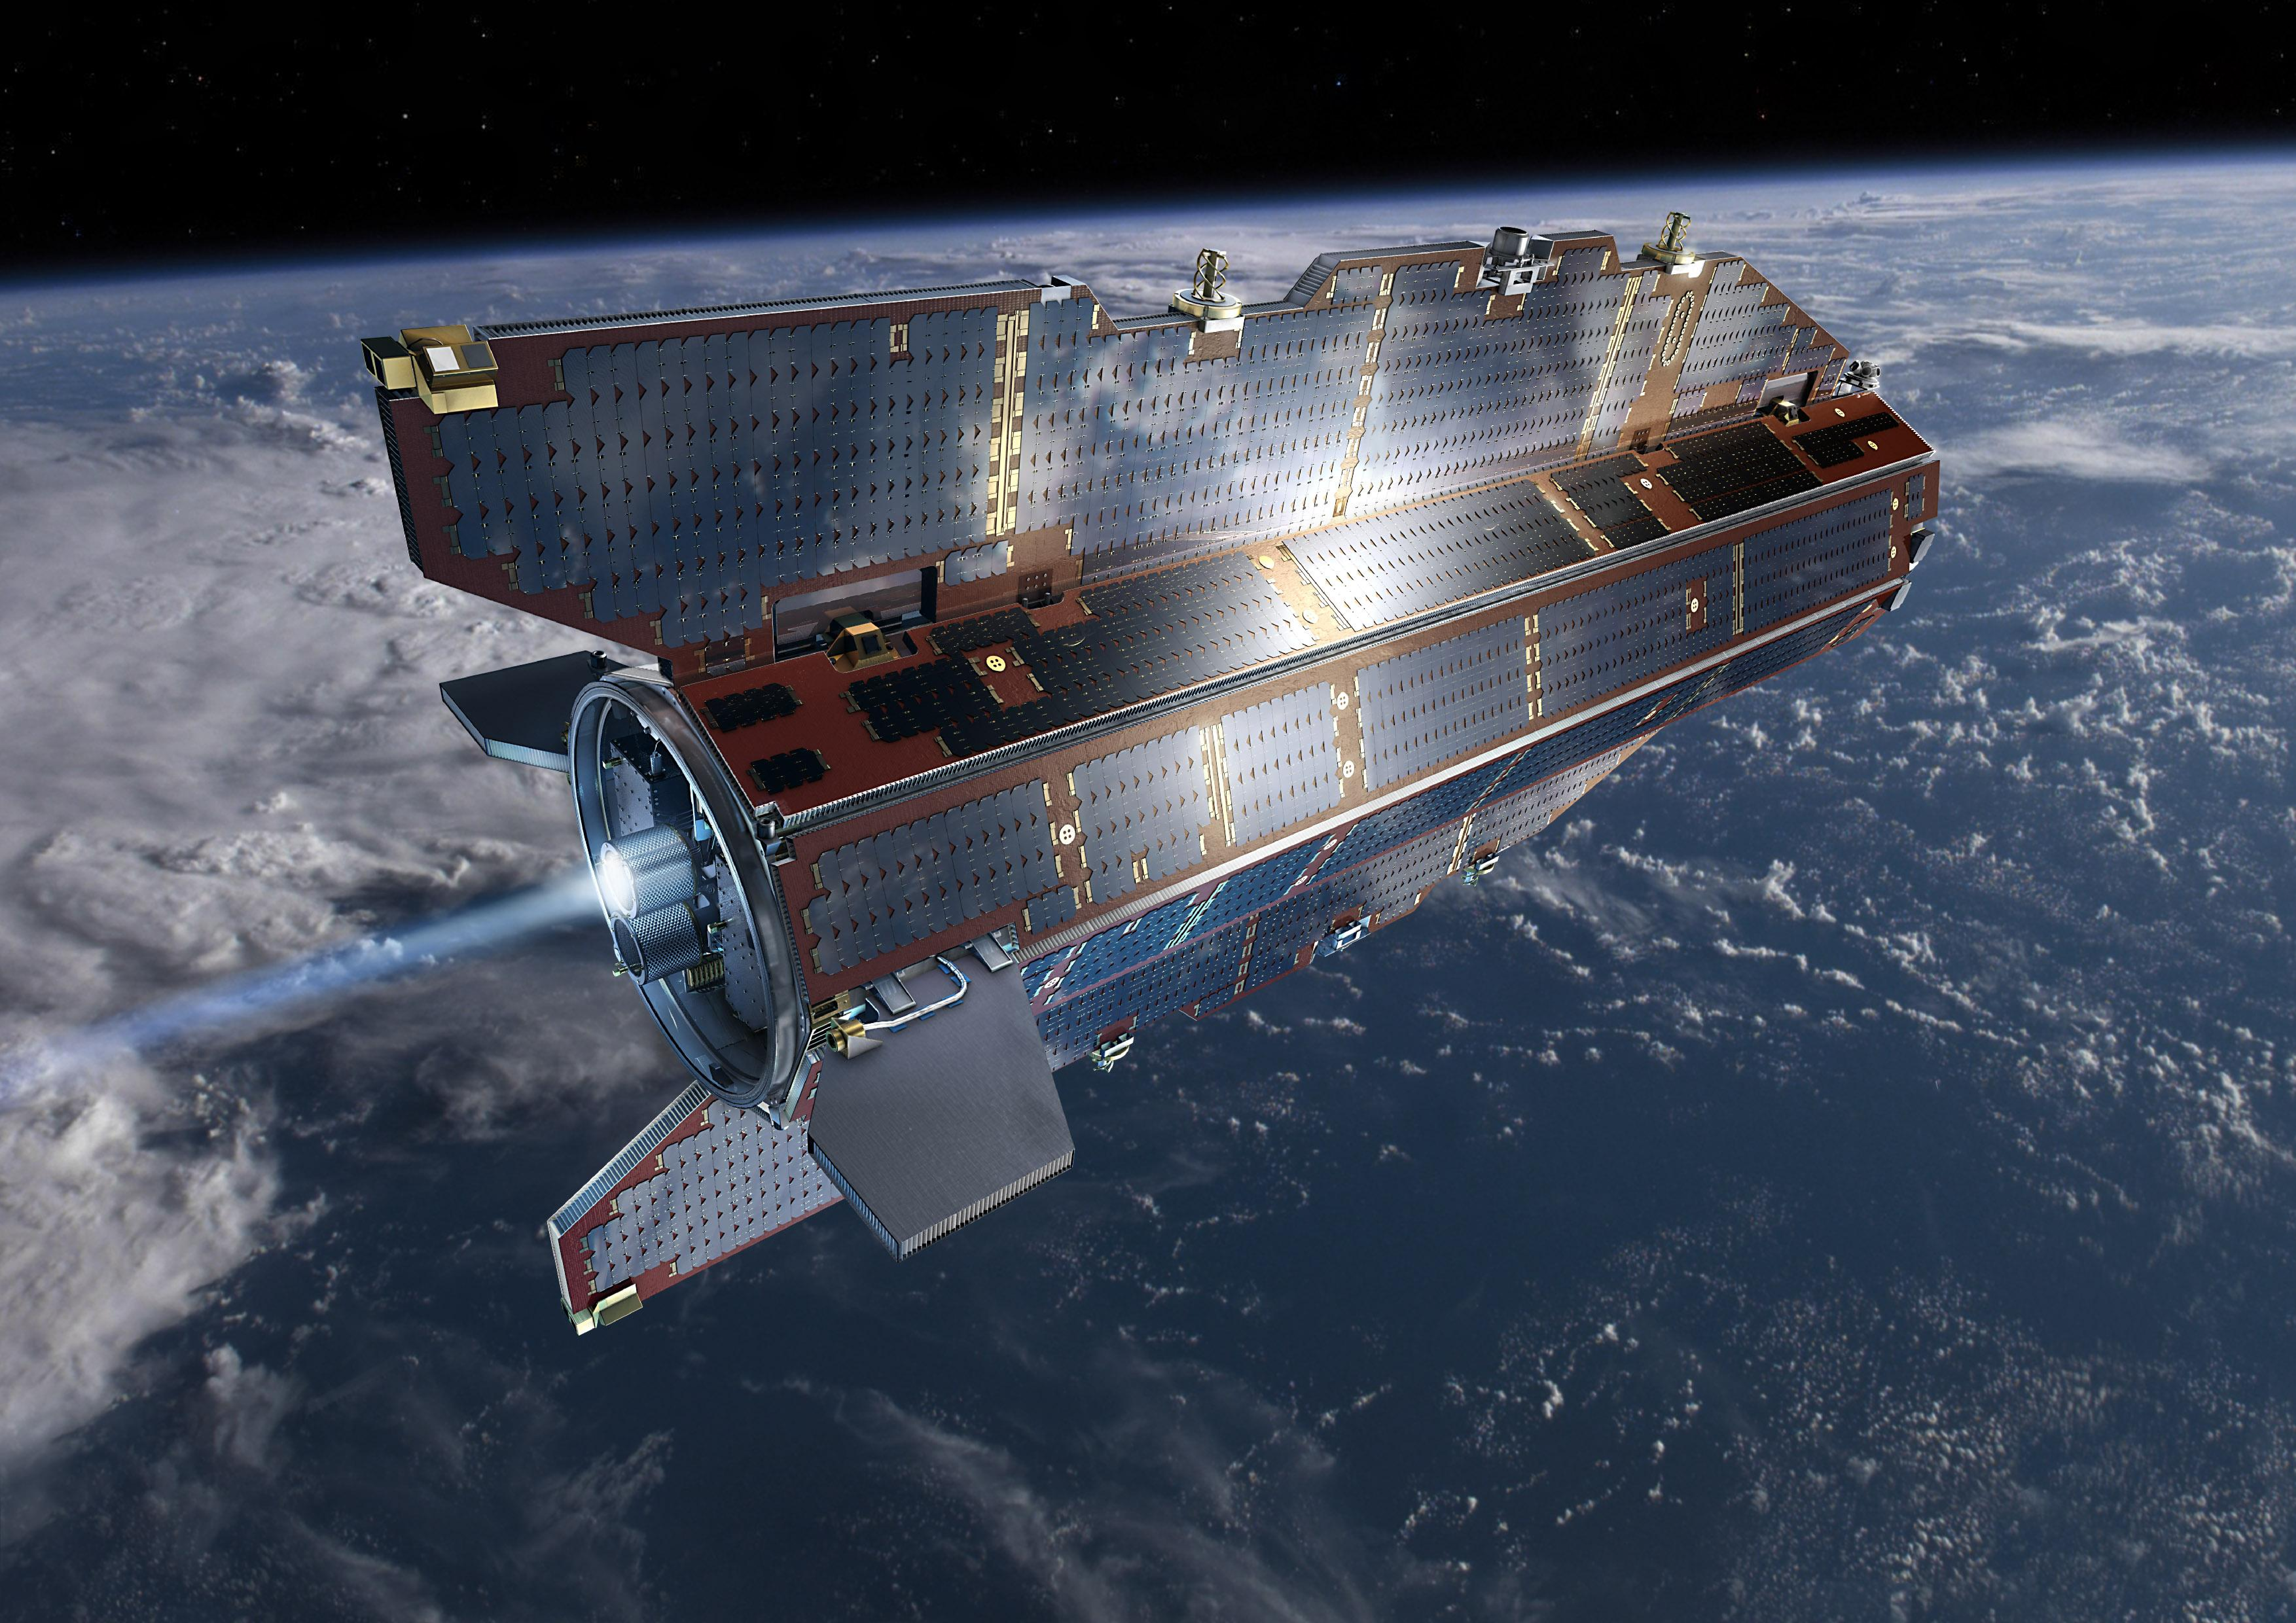
\includegraphics[width=\linewidth]{papers/planet/pictures/goce.pdf}
    \caption{Sattelit aus der GOCE Mission \cite{planet:gocepic}
        \label{planet:fig:goce}}
\end{figure}

Der Gravity Field and Steady-State Ocean Circulation Explorer (GOCE) ist ein Satellit, der im März 2009 von der Europäischen Weltraumorganisation ESA ins Weltall geschickt wurde.
GOCE umkreist die Erde in einer erdnahen Umlaufbahn von nur 260\,km höhe, um das Schwerefeld der Erde mit bisher unerreichter Genauigkeit und räumlicher Auflösung zu erfassen.
Dafür nutzt GOCE einen Gradiometer unterstützt durch GPS um zusätzlich in Echtzeit die Navigation der Umlaufbahn aufzuzeichnen.

\begin{figure}[h]
    \centering
    \includegraphics[width=\linewidth]{papers/planet/pictures/geoid.pdf}
    \caption{Darstellung des Gravitationsfeld der Erde \cite{planet:geoidpic}
        \label{planet:fig:geoid}}
\end{figure}


